\section{\LARGE{Preparazione di:  terreno LB solido, cellule competenti e piastre LB-agar }}

\vspace{0.6cm}


\subsection{Sommario}

\subsubsection{Scopo}

Quest'esperienza in laboratorio si divide in tre fasi: Una prima fase che consiste nella preparazione del terreno di cultura dove andranno a crescere le nostre cellule batteriche; Una seconda fase consistente nella preparazione delle cellule competenti; E infine l'ultima fase consiste nella preparazione delle piastre di LB-agar, dove andremo a mettere il terreno e infine dove cresceranno i nostri batteri.


\subsubsection{Cenni teorici}

\textbf{Colture batteriche}
\vspace{0.3cm}

All'interno dei laboratori, i ceppi che comunemente si usano sono dei ceppi che derivano dal batterio di E.coli, che è un batterio gram negativo non patogeno, che viene selezionato e modificato.
A seconda del genotipo, cioè con mutazioni su particolari geni o introduzione di geni estranei, vengono utilizzati per diversi scopi, però in generale si possono dividere in questo modo:
\begin{itemize}
  \item Ceppi di propagazione, atti al clonaggio o alla propagazione di plasmidi;

  \item Ceppi di espressione, atti ad esprimere le proteine ricombinanti.

\end{itemize}

\begin{figure}[H]

  \centering
  \subfloat{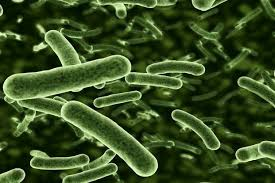
\includegraphics[width=0.3\textwidth]{./immagini/e_coli.jpeg}} \quad
  \subfloat{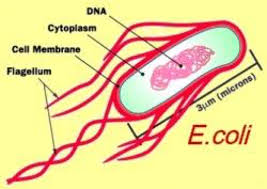
\includegraphics[width=0.3\textwidth]{./immagini/e_coli1.jpeg}}
  \caption{vista al microscopio del batterio di Eschericchia coli (destra) e suddivisione di questo batterio (sinistra)}
  \label{e_coli}

\end{figure}

\textbf{Terreni di cultura}
\vspace{0.3cm}

I terreni di cultura, sono le soluzioni solide o liquide contenenti sostanze nutritive su cui è possibile crescere delle cellule eucariotiche (come E.coli) e procariotiche.
Una possibile suddivisione può essere:

\begin{tabular}{ll}
\hline
\multicolumn{1}{c}{Stato fisico}

& -\textbf{LIQUIDI}: componenti sciolti in acqua e sterilizzati; \\ \cline{1-1} &usati per crescita delle cellule;\\&  espressione di proteine ricombinanti ecc..\\

& -\textbf{SOLIDI}:  possono essere naturalmente tali (terreno alla patata)\\ & o vengono solidificati per aggiunta di un agente gelificante (agar, gelatina). \\ &selezioni di cloni mediate isolamento di
singole colonie, propagazione \\ & delle colonie o della linea cellulare \\

\hline
\multicolumn{1}{c}{Costituzione chimica}

& -\textbf{MINIMI}: Per la crescita dei soli batteri autotrofi. Gli elementi \\ \cline{1-1} & essenziali (N, C, S, P) sono presenti come sali inorganici\\ & in composizione e quantità note.\\
& -\textbf{SINTETICI}(Definiti) : nota la formulazione chimica di ogni ingrediente; \\ & le singole sostanze di cui il batterio necessita sono presenti in quantità note.\\
& -\textbf{COMPLESSI}: Ignota l’esatta composizione chimica delle sostanze nutritive \\ & (estratto di carne di bue, cuore, cervello, ecc.), benché chimicamente non definite.\\ & Comprendono la maggior parte dei terreni usati in laboratorio. \\ & in  questa sezone c'è il terreno LB(Luria Bertani medium).\\ &  Questi terreni sono utilizzati per la crescita di cellule e per l’espressione
\\ & di proteine ricombinanti non modificate.\\

\hline
\multicolumn{1}{c}{Funzione}

& -\textbf{ARRICCHIMENTO}(ELETTIVI): la specie microbica di interesse vi cresce in \\ \cline{1-1} & un tempo assai più breve rispetto ad altre specie microbiche.\\
& -\textbf{SELETTIVI}: Contengono sostanze batteriostatiche (sali biliari, NaCl) \\ &  a concentrazione nota che inibiscono o rallentano lo sviluppo \\ & di molte specie microbiche. \\ &  Utilizzati per isolare specifici microrganismi da campioni altamente contaminati.\\
& -\textbf{DIFFERENZIALI}: Contengono sostanze indicatrici di particolari reazioni \\ & biochimiche che avvengono nel terreno stesso. \\ & Usati per la identificazione di specifici microrganismi.\\


\end{tabular}

\textbf{Piastra agar}
\vspace{0.3cm}

Una \textbf{piastra Agar} è un disco di Petri sterile che contiene nutrimenti di crescita (tipicamente agar + nutrienti) usati per coltivare micro-organismi o piccole piante.
componenti di crescita selettivi, si possono aggiungere agli altri come per esempo antibiotici.




\subsubsection{Materiali utilizzati}

\begin{itemize}
	\item Guanti in lattice
	\item Micropipette (100-1000 e 2-200 microlitri)
	\item Bottiglia da laboratorio
  \item Piastre di Petri
	\item Forno a micronde
  \item provetta Falcon da 50mL
  \item provetta eppendorf 2mL

\end{itemize}

\subsubsection{Soluzioni utilizzate}

\begin{itemize}

  \item Soluzione Buffer I:
  \begin{enumerate}
    \item RbCl 12 g/l (0.6g)
    \item MnCl*4H\textsubscript{2}O 9.9 g/l (0.49g)
    \item 1.5 ml di una soluzione di KAc 1M a pH 7.5
    \item CaCl\textsubscript{2}*2H\textsubscript{2}O 1.5 g/l (0.075g)
    \item Glicerolo 150 g/l (7.5g)
    \item Si porta a pH 5.8 con HAc, si porta a volume (50ml) con acqua milliQ e si filtra con una membrana a pori di 0.22 \SI{250}{\micro\liter} sotto cappa.
  \end{enumerate}
  \item Soluzione Buffer II:
  \begin{enumerate}
    \item 0.4 ml di una soluzione di MOPS 0.5 M a pH 6.8
    \item RbCl 1.2 g/l (0.025g)
    \item CaCl\textsubscript{2}*2H\textsubscript{2}O 11 g/l (0.22g)
    \item Glicerolo 150 g/l (3g)
    \item Si porta a volume (20ml) con acqua milliQ e si filtra con una membrana con pori di 0.22 \SI{250}{\micro\liter} sotto cappa.
  \end{enumerate}

\end{itemize}

\subsection{Procedimento}

\subsubsection{Preparazione del terreno LS-solido}

La composizione del terreno LB(Luria-Bertani) medium è di :

\begin{itemize}
  \item 1\% Tryptone
  \item 0.5\% Estratto di lievito
  \item 0.5\% inattaccabile
  \item 1.5\% Agar batteriologico
\end{itemize}

Per la preparazione di questo terreno bisogna eseguire questi passaggi:

\begin{enumerate}

	\item Pesare le quantità necessarie cioè prendere: 0.5g di tryptone, 0.25g di estratto di lievito, 0.025g di NaCl e 0.75g di agar batteriologico e metterle in una beuta portando a volume 50mL con acqua distillata.
  \item Attaccare alla mia bottiglia da laboratorio un autoclave, cioè un pezzo di scotch ma che si va a marcare quando la sua temperatura raggiunge i 100°C, questo serve per sapere se la nostra bottiglia, una volta inserita nella chiusura autoclave raggiunge la temperatura adatta per la nostra reazione.

	\item Poratare la Bottiglia all'interno dell' autoclave, cioè una macchina che è molto simile al funzionamento di una pentola a pressione, nella quale il contenuto delle bottigliepotrà raggiungere la giusta temperatura per la reazione.

  \begin{figure}[H]
		\centering
		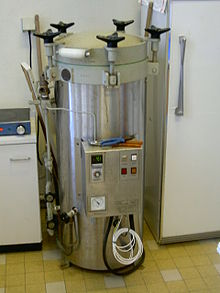
\includegraphics[width=0.3\textwidth]{./immagini/autoclave.JPG}
		\caption{Autoclave}
		\label{autoclave}

	\end{figure}


\end{enumerate}



\subsubsection{Preparazione delle cellule competenti}


\begin{enumerate}

	\item Prelevare sotto cappa biologica 5 mL di una coltura di cellule i E. coli DH5a ed OD 600 di 0.3-0.4 e trasferirli in una provetta Falcon da 50 mL sterile;

  \item Portare la provetta Falcon con le cellule di E.coli all'interno della centrifuga, e centrifugare per 5 minuti a 3000 g, a 4°C;

  \item Prelevare la falcon centrifugata ed eliminare il surnatante, semplicemente rovesciando il contenuto. Le nostre cellule staranno ancorate in fondo alla provetta Falcon raggruppate, formando un pellet;

  \item Risospendere le cellule in 0.8mL di buffer I;

  \item Trasferire il contenuto in una provetta eppendorf da 2mL sotto cappa biologica;

  \item Incubare in ghiaccio per 15 minuti;

  \item Passati i 15 minuti si riprende la provetta eppendorf e la si fa centrifugare per 5 minuti a 3000g a 4°C;

  \item Andare sotto cappa bilogica per eliminare il surnatante e risospendere le cellule in \SI{400}{\micro\liter} di buffer II

  \item Congelare in N\textsubscript2 liquido e conservare a -80°C, questo passaggio viene effettuato con N\textsubscript2 liquido perchè il passaggio di temperatura deve avvenire molto velocemente per garantire che le nostre cellule diventino competenti;

\end{enumerate}

\subsubsection{Preparazione delle piastre di LB-agar}

Una volta che le bottiglie all'interno dell'autoclave sono state tolte, si prendono senza farle raffreddare troppo perchè senò la miscla si solidifica ed andando sotto cappa biologica
aggiungiamo 100 \SI{100}{\micro\gram}/ml di ampicillina (\SI{50}{\micro\liter} dello stock 1000X). Una volta mescolato abbastanza, Si versa il terreno dalle bottiglie alle due pistre di Petri, Lasciandole
aperte sotto cappa fino a che l'agar non solidifica. Una volta che l'agar si è solidificato si conservano a 4°C.


\subsection{Risultati e Conclusioni}

Durante questa esperienza, abbiamo capito come preparare un terreno di coltura batterico, specialemtne un terreno solido LB, contenente ampicillina, che nella prossima esperienza capiremo a cosa serve;
Abbiamo preparato poi delle cellule competenti, in grado di poter integrare del materiale genetico proveniente da un ambiente extracellulare;
Ed infine abbiamo perparato una piastra di Petri con il nostro terreno mixato in precedenza.
